%%%%%%%%%%%%%%%%%%%%%%%%%%%%%%%%%%%%%%%%%%%%%%%%%%%%%%%%%%%%%%%%%%%%%%%%%%%%%%%%
%2345678901234567890123456789012345678901234567890123456789012345678901234567890
%        1         2         3         4         5         6         7         8

%\documentclass[letterpaper, 10 pt, conference]{ieeeconf}  % Comment this line out if you need a4paper

\documentclass[a4paper, 10pt, conference]{ieeeconf}      % Use this line for a4 paper

%\IEEEoverridecommandlockouts                              % This command is only needed if 
                                                          % you want to use the \thanks command

\overrideIEEEmargins                                      % Needed to meet printer requirements.

% The following packages can be found on http:\\www.ctan.org
\usepackage{subfigure}
\usepackage[OT1]{fontenc} 
\usepackage{graphicx} % for pdf, bitmapped graphics files
\usepackage{multirow}
%\usepackage{epsfig} % for postscript graphics files
%\usepackage{mathptmx} % assumes new font selection scheme installed
%\usepackage{times} % assumes new font selection scheme installed
%\usepackage{amsmath} % assumes amsmath package installed
%\usepackage{amssymb}  % assumes amsmath package installed

\title{\LARGE \bf
Off-Road Drivable Area Extraction Using 3D LiDAR Data
}


\author{\authorblockN
	{Biao Gao\authorrefmark{1},
		Anran Xu\authorrefmark{1}, 
		Yancheng Pan\authorrefmark{1},
		Xijun Zhao\authorrefmark{2},
		Wen Yao\authorrefmark{2},
		Huijing Zhao\authorrefmark{1}}
	\authorblockA{\authorrefmark{1}Peking University, Beijing, China}
	\authorblockA{\authorrefmark{2}China North Vehicle Research Institute, Beijing, China}}

\begin{document}


\maketitle


%%%%%%%%%%%%%%%%%%%%%%%%%%%%%%%%%%%%%%%%%%%%%%%%%%%%%%%%%%%%%%%%%%%%%%%%%%%%%%%%
\begin{abstract}
	
nothing.

\end{abstract}


%%%%%%%%%%%%%%%%%%%%%%%%%%%%%%%%%%%%%%%%%%%%%%%%%%%%%%%%%%%%%%%%%%%%%%%%%%%%%%%%
\section{INTRODUCTION}

nothing.

\section{RELATED WORKS}

nothing.

\begin{figure}[ht]
	\centering
	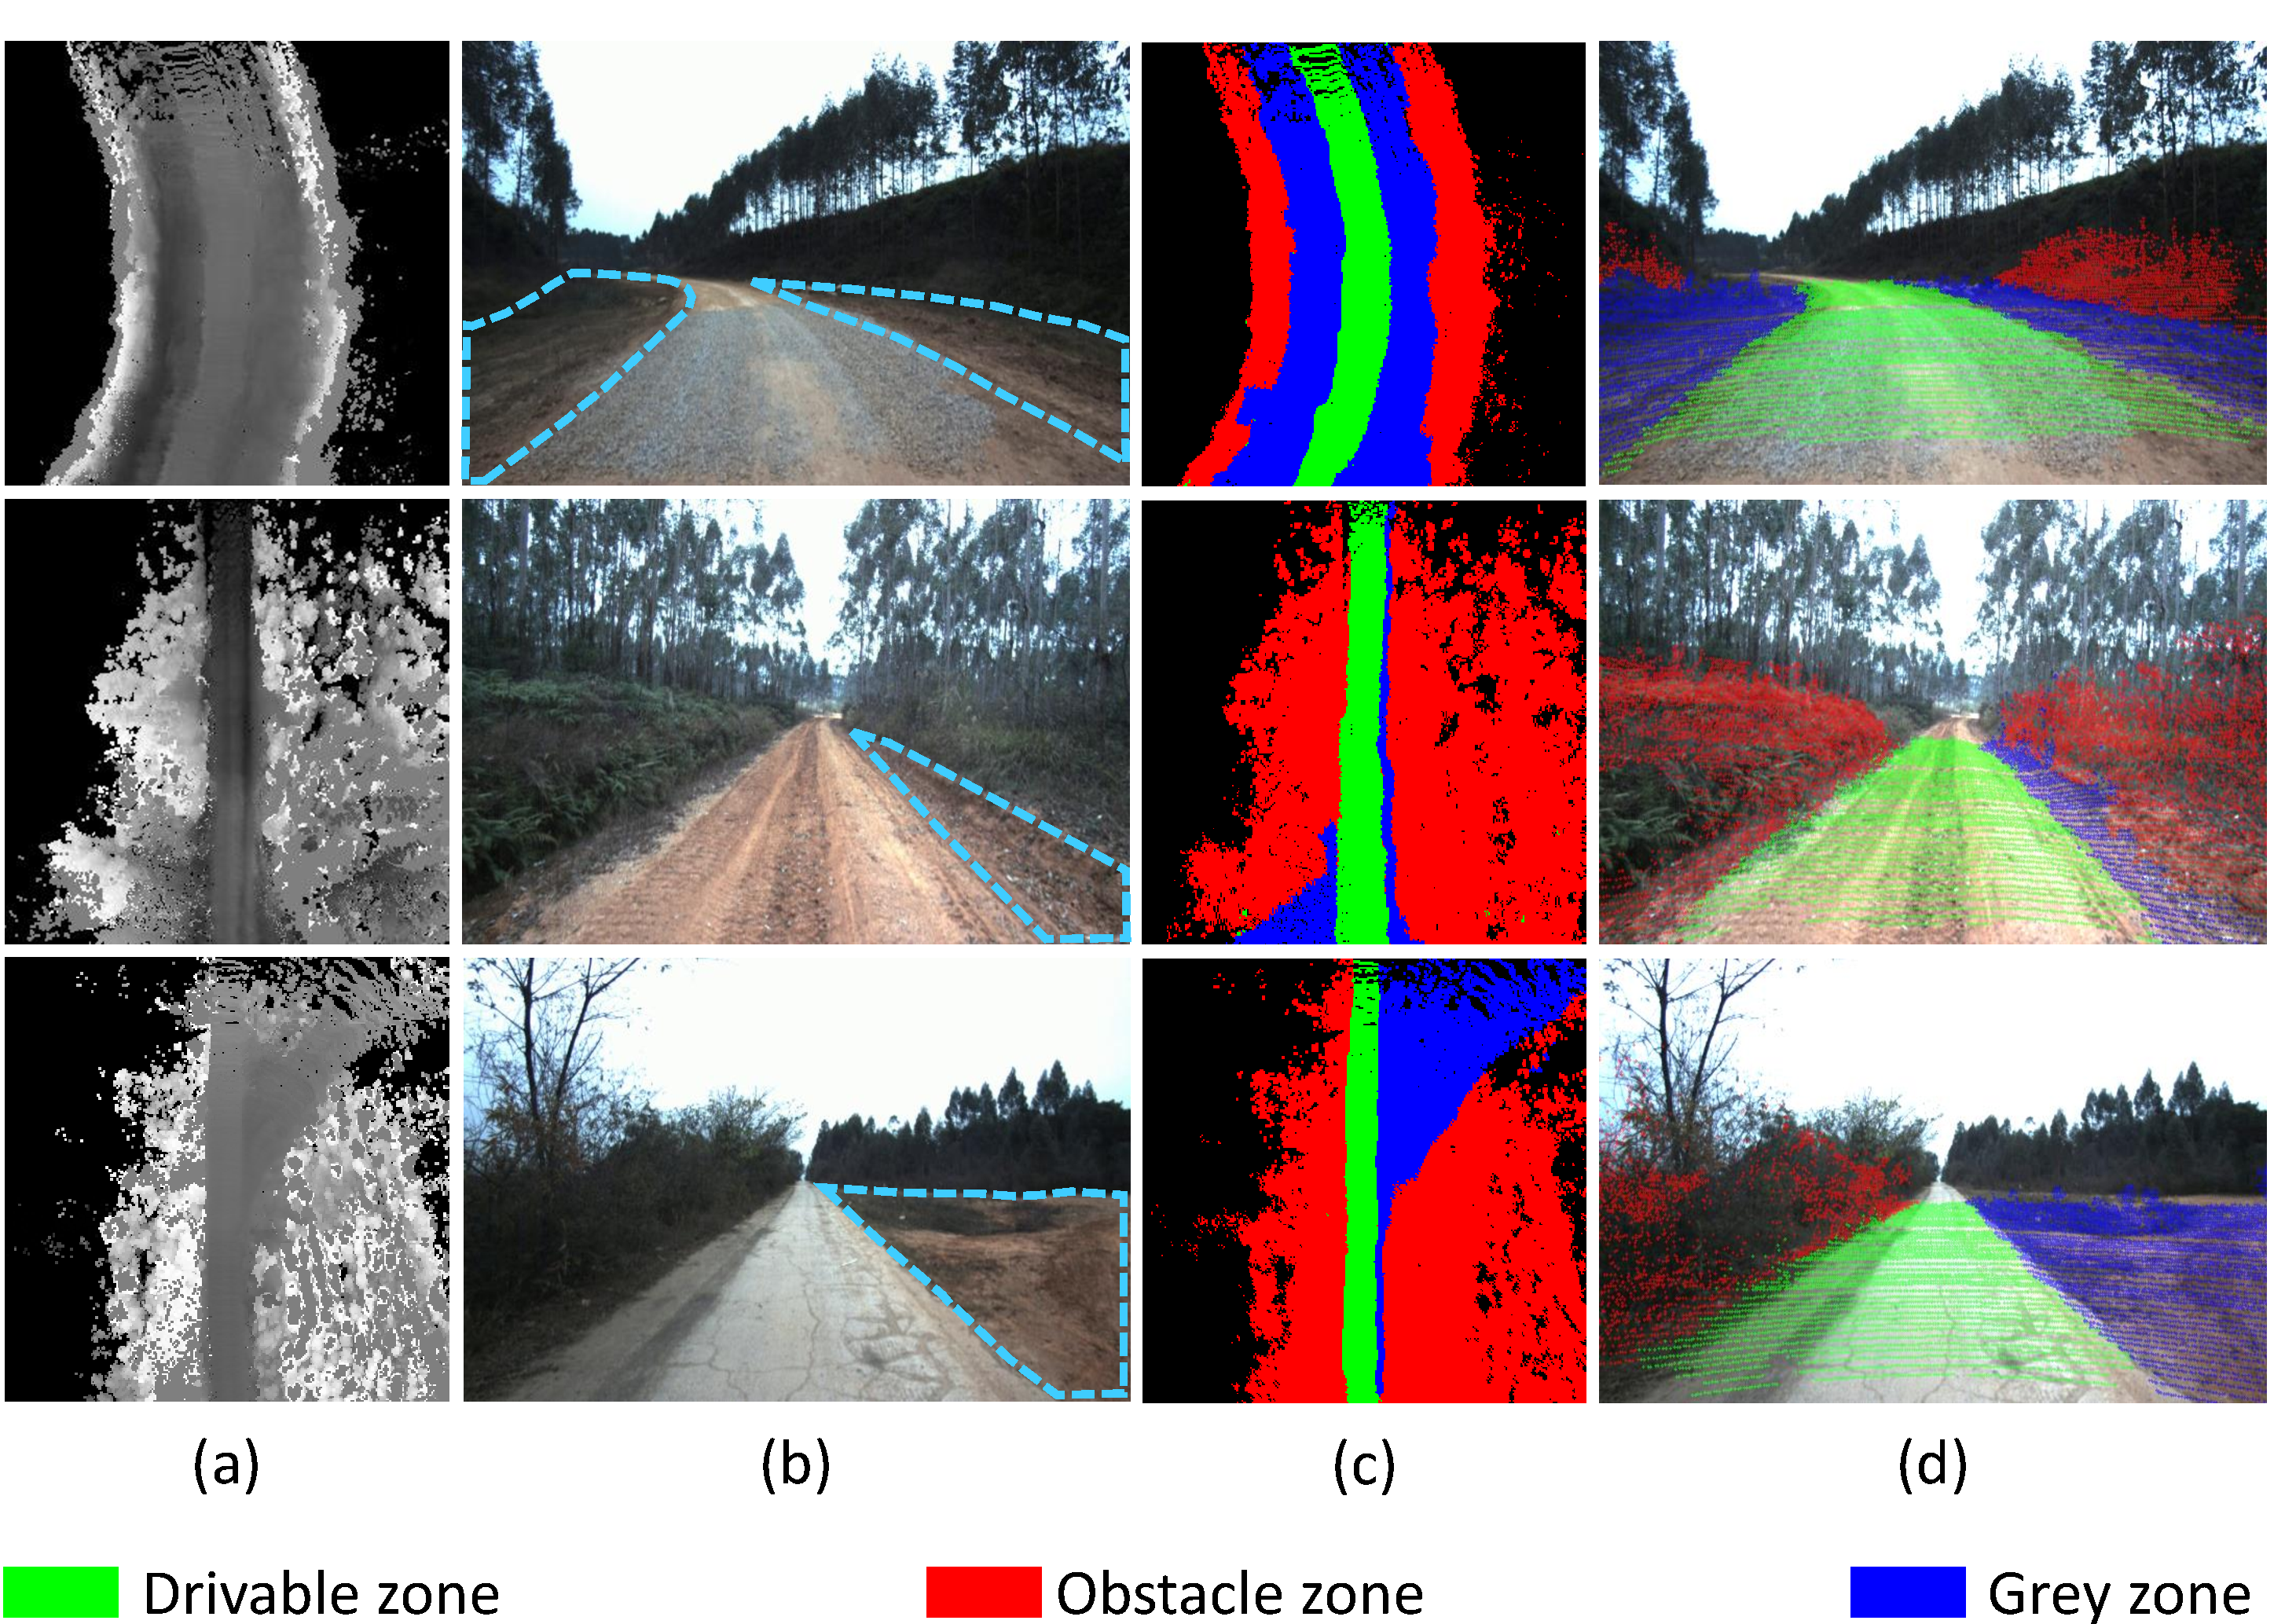
\includegraphics[scale=0.175]{offRoadExample.pdf}
	\caption{The ambiguities in off-road drivable area extraction. (a) Input LiDAR data in bird's-eye view. (b) Image reference of input data. (c) Human annotation. (d) Projected point clouds in camera coordinate.}
\end{figure}

\section{METHODOLOGY}

\subsection{Problem Definition}

The origin data are point clouds from 3D LiDAR sensor, which are denoted as $PC={\{pt_i\}}_{0\le i<N}$, where $N$ is the number of points. In order to get a bird's-eye view height map with denser point clouds, we aggregate point clouds from a few frames to one height map $X$ as our networks' input. $X=\{x_{j,k}\}_{0\le j<H,0\le k<W}$ is in the size of $H\times W$ and $x_{j,k}$ means the physical height of pixel $(j,k)$.

We let $G=\{g_{j,k}\}_{0\le j<H,0\le k<W}$ denote human annotated ground truth, where $g_{j,k}\in \{unknown,drivable\ zone,obstacle\ zone,gray\ zone\}$

\subsection{Data Processing}
% ??????

\subsection{Drivable Area Extraction / Network Architecture}
% ???????

\begin{figure*}[h]
	\centering
	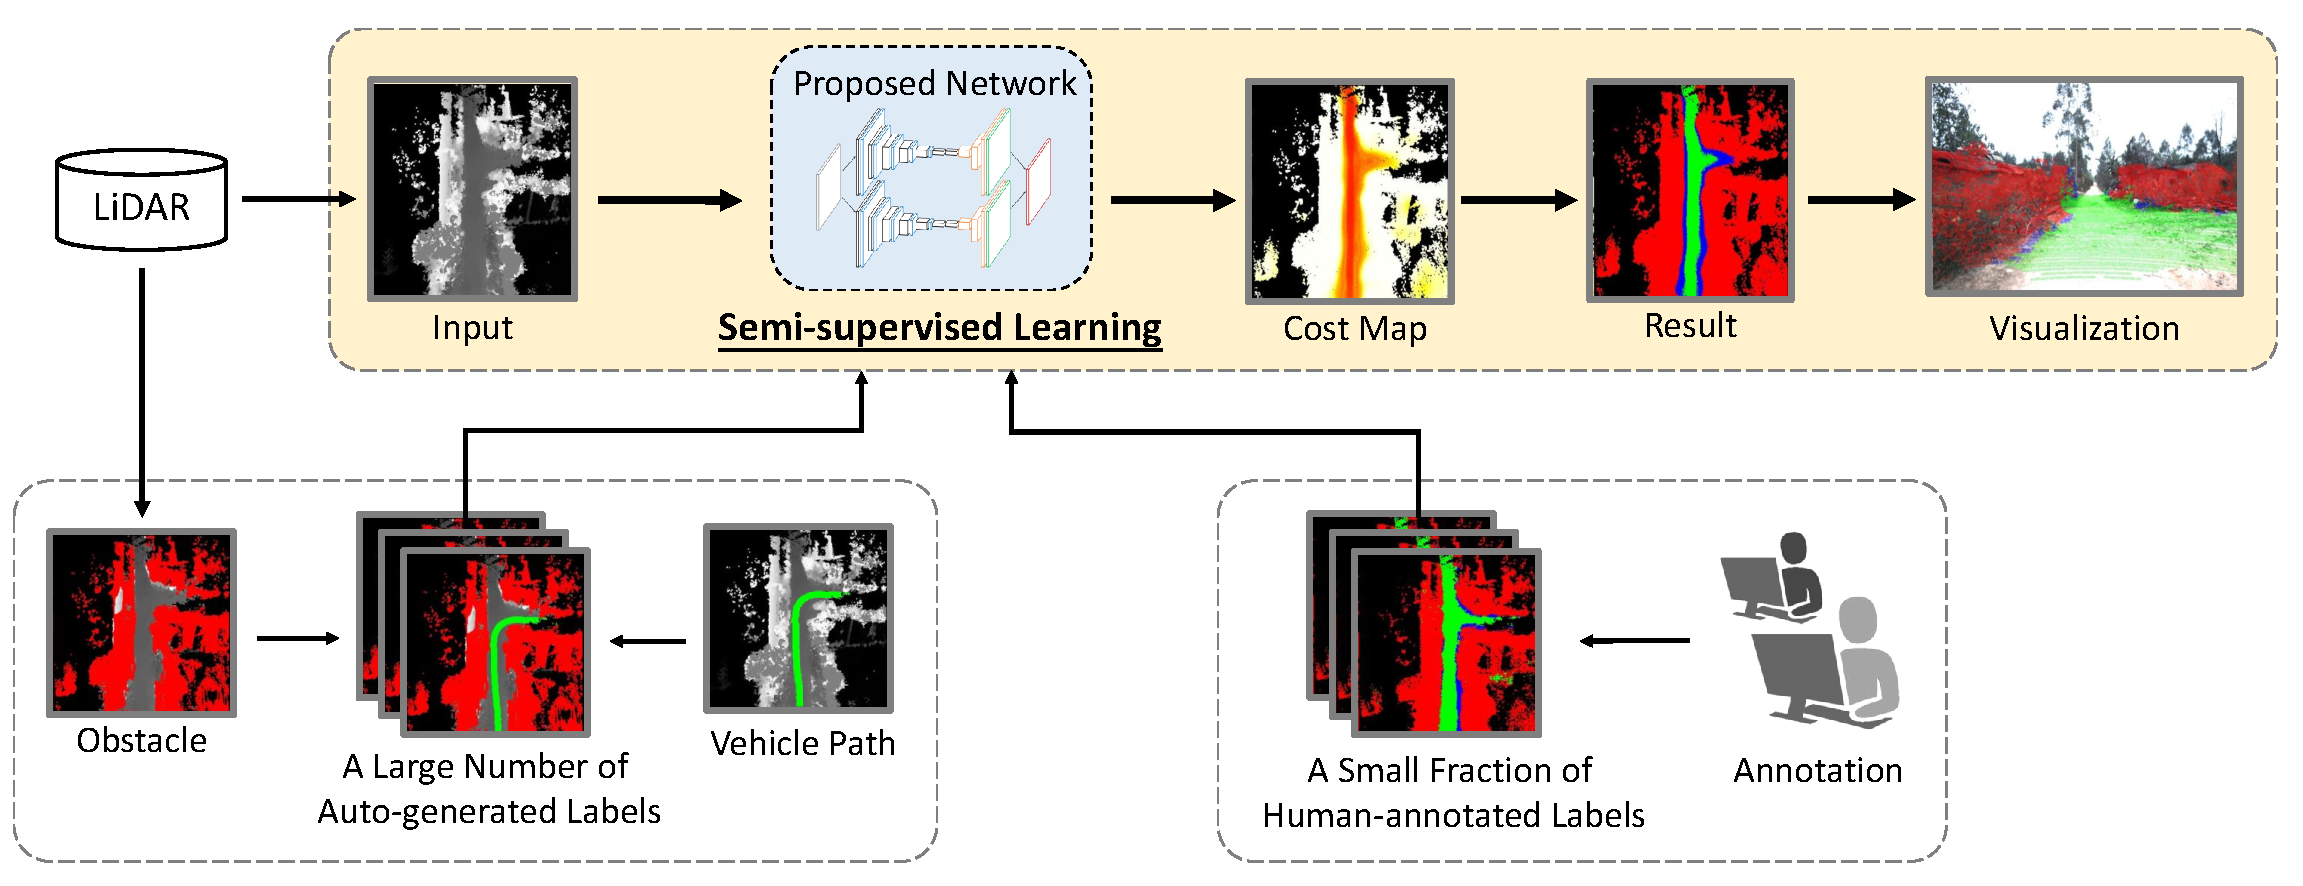
\includegraphics[scale=0.4]{framework.pdf}
	\caption{Overview of the proposed off-road drivable area extraction framework}
	\label{framework_fig}
\end{figure*}

\begin{figure}[!h]
	\centering
	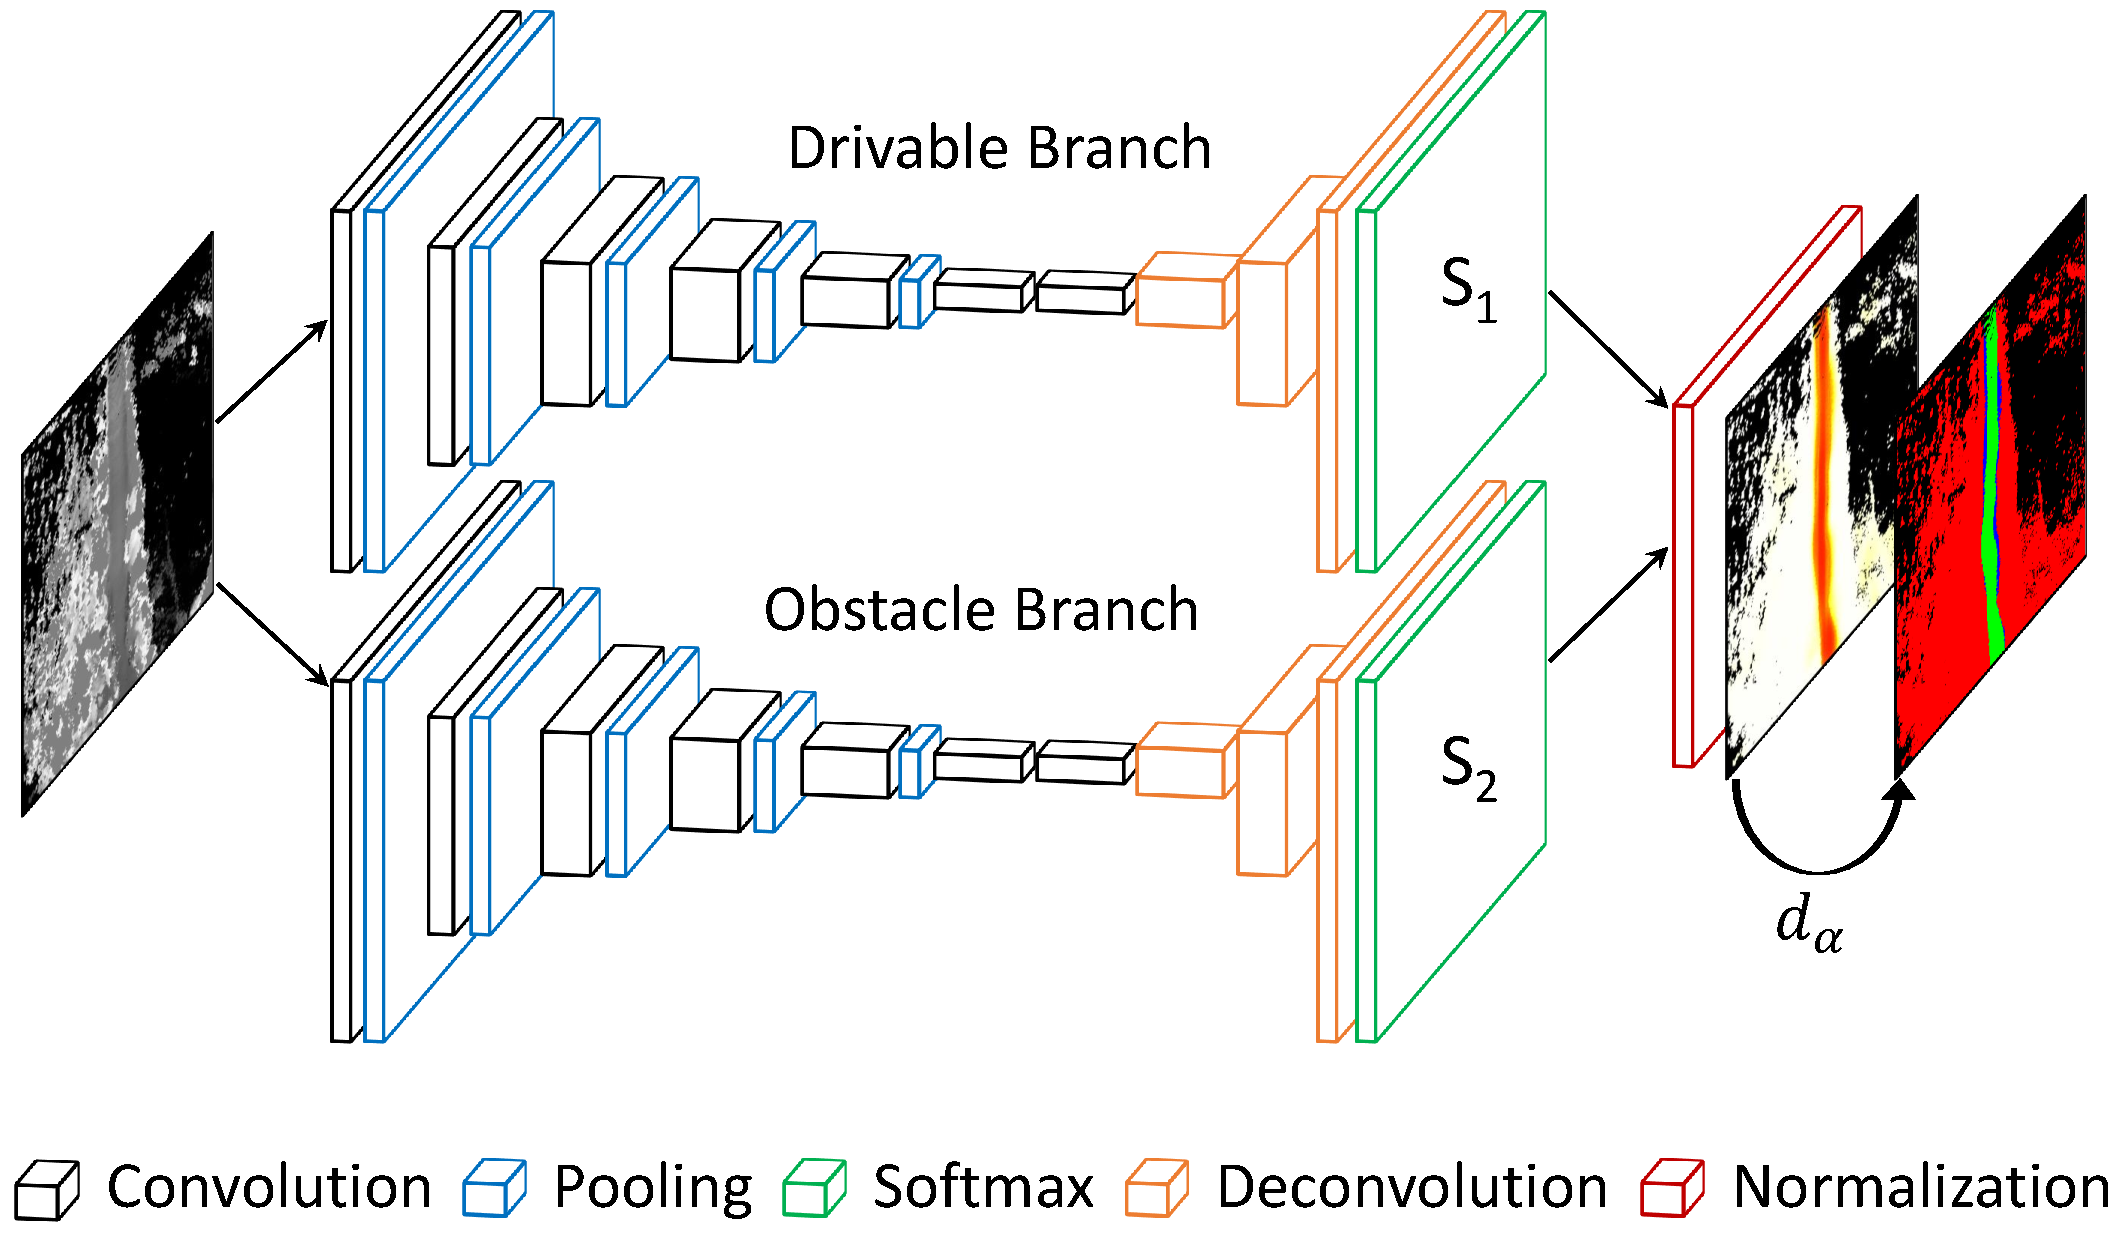
\includegraphics[scale=0.24]{network.pdf}
	\caption{Framework}
	\label{network_fig}
\end{figure}

\begin{equation}
	L^{br}=-\sum_{i}{y_i^{br} \log{P(y_i^{br}|\Theta^{br})}} \ ,\quad br \in \{dri, obs\}
\end{equation}

\[
	y_i^{br}= 
	\left\{
		\begin{array}{ll}
			\vec{br}, &\quad if \ y_i = \vec{gre} \\ 
			y_i &\quad if \ y_i \in \{\vec{dri},\vec{obs} \} \\
		\end{array}
	\right.
\]

\begin{equation}
L^{br}_{semi}=-\lambda \sum_{j}{\widetilde{y_j^{br}} \log{P(y_j^{br}|\Theta^{br})}} \ ,\  br \in \{dri, obs\}
\end{equation}

\[
\widetilde{y_j} \in \widetilde{Y},\ \  \mbox{Auto-generated Labels}
\]

\[
S= 
\left\{
\begin{array}{ccc}
S_1, &\  if \ S_1>\alpha_1 \\ 
1-S_2, &\ if \ S_2>\alpha_2 \\
\frac{1-S_2}{1-S_1 + 1-S_2}, &\ otherwise
\end{array}
\right.
\]
\subsection{Cost Map Generation}

\subsection{Weakly and Semi Supervised Extraction}

\section{IMPLEMENTATION DETAILS}

\subsection{Training Setup}

\subsection{Ground Truth Labeling}

\subsection{Evaluation}

\section{EXPERIMENTAL RESULTS}

\subsection{Data set}

\subsection{Proposed Method Results}

\begin{figure*}[ht]
	\centering
	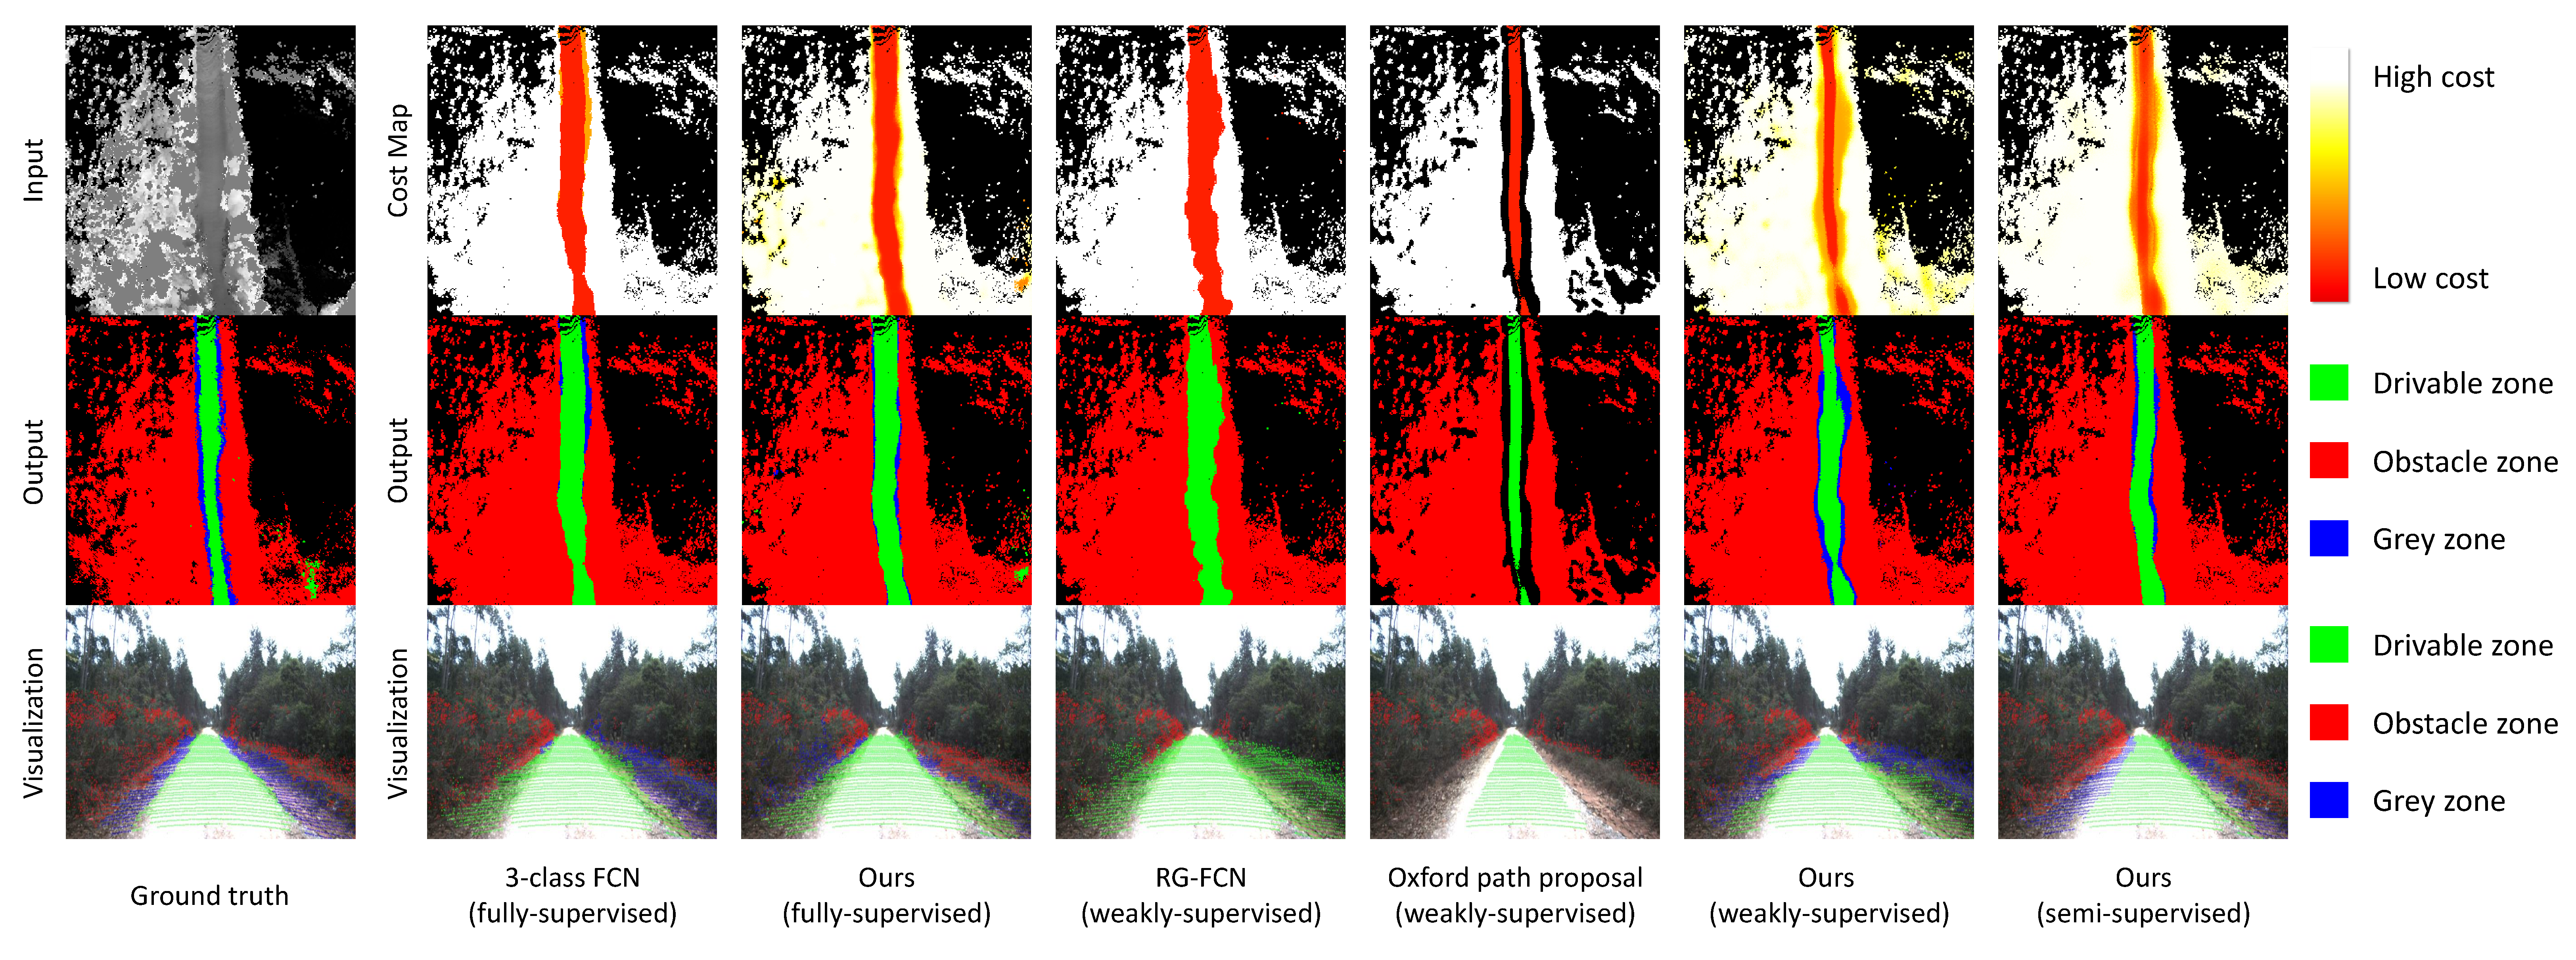
\includegraphics[scale=0.17]{straightRoad.pdf}
	\caption{Qualitative results at straight road scene.}
	\label{straight_road_fig}
\end{figure*}

\begin{figure*}[h]
	\centering
	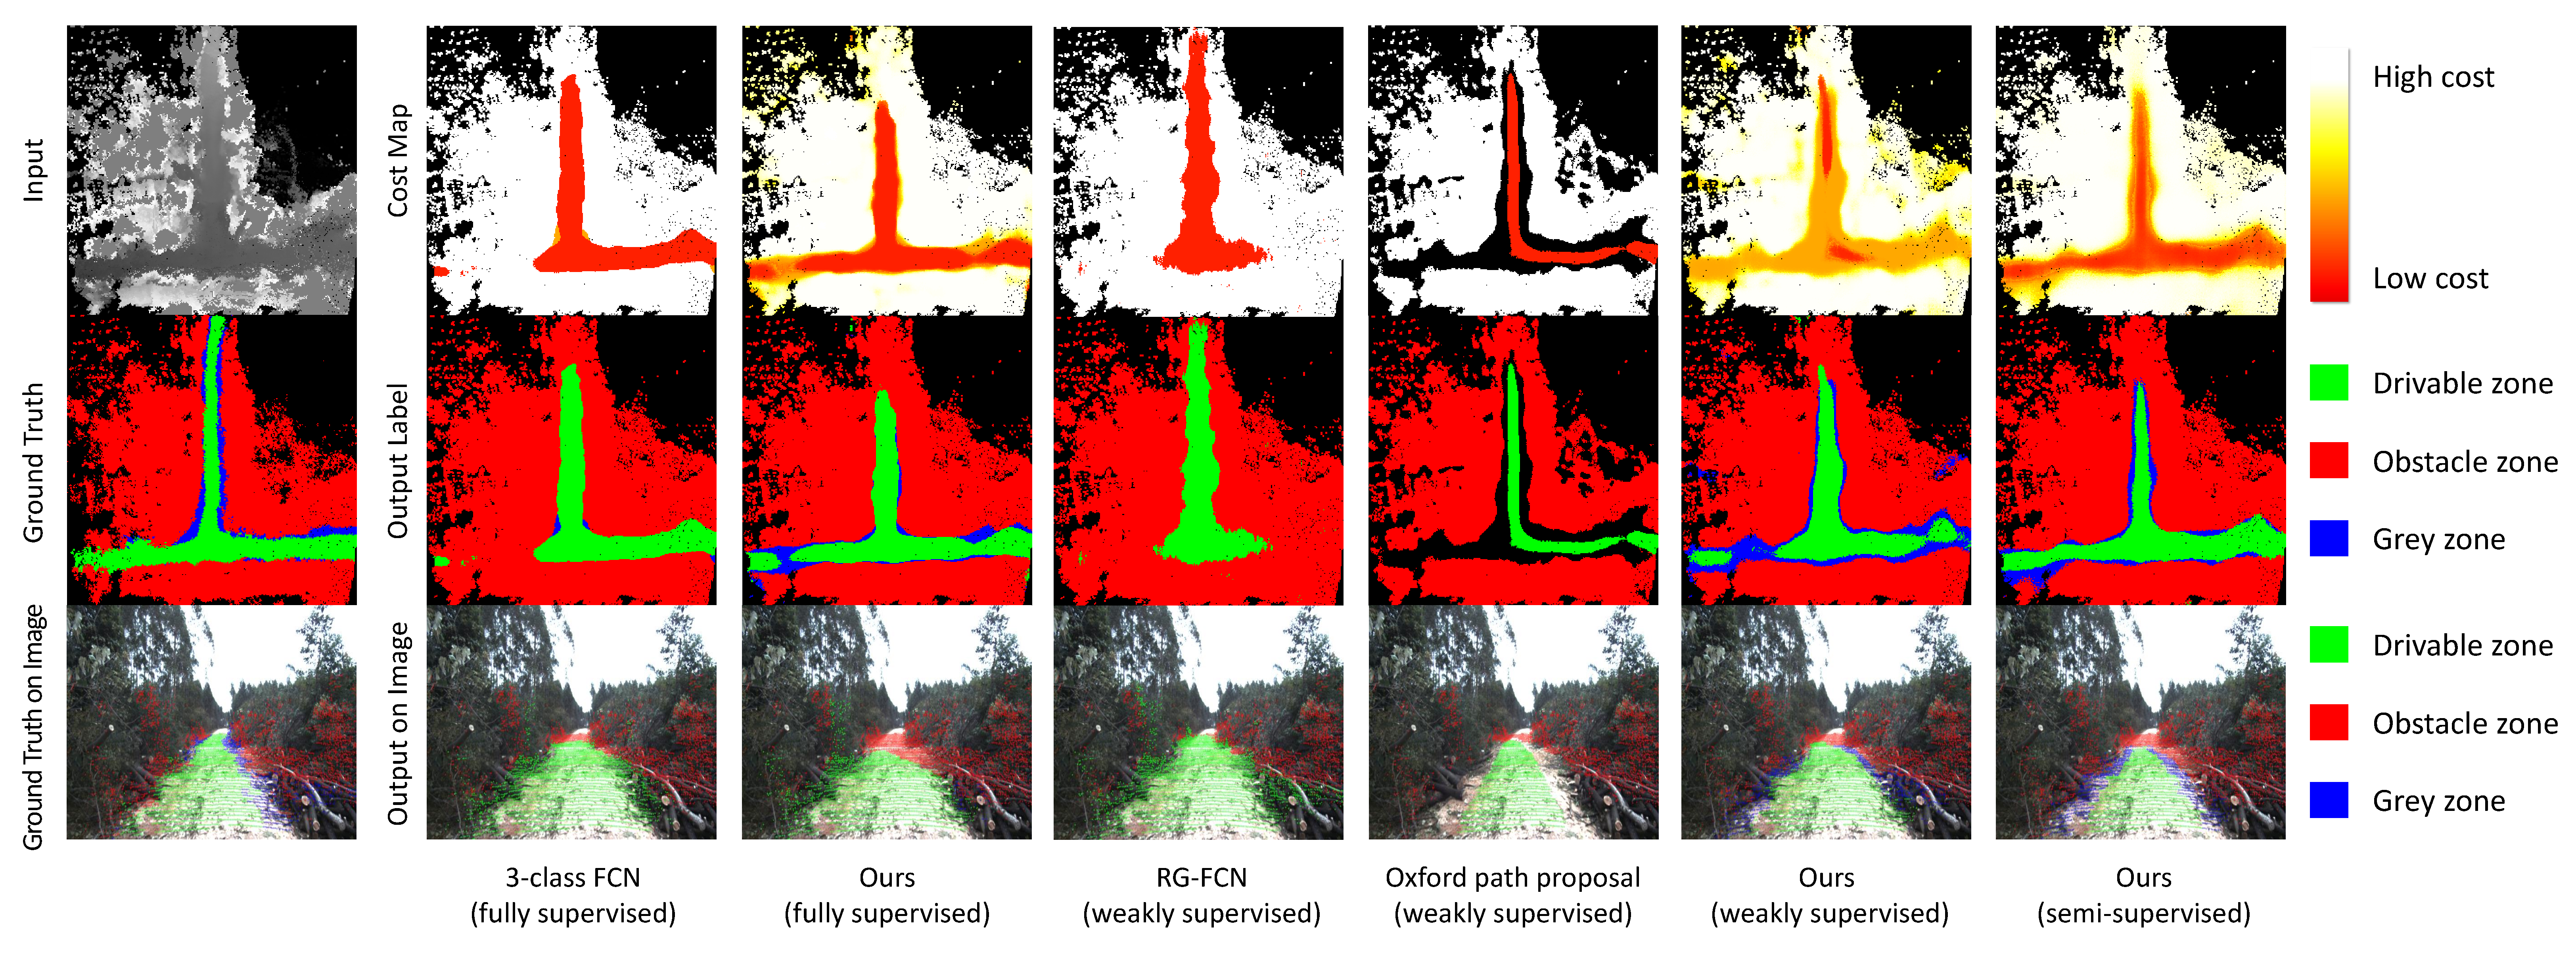
\includegraphics[scale=0.17]{crossRoad.pdf}
	\caption{Qualitative results at cross road scene.}
	\label{cross_road_fig}
\end{figure*}


\begin{figure}[h]
	\centering
	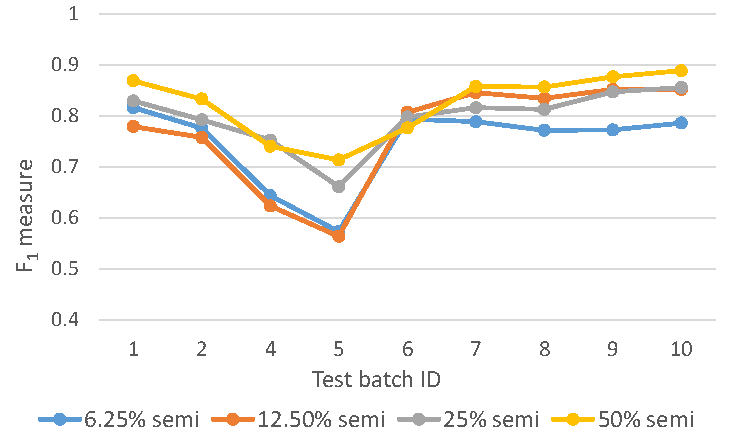
\includegraphics[scale=0.6]{semiSupvisedResult.pdf}
	\caption{Quantitative comparison on test set.}
	\label{semi_curve_fig}
\end{figure}

\begin{table*}
	\caption{Evaluation Measures}
	\label{evaluation_table}
	\centering
	\renewcommand{\arraystretch}{1.7}
	\begin{tabular}{cclccl}
		\hline
		\multicolumn{3}{c|}{Drivable Zone}                                                                                                    & \multicolumn{3}{c}{Obstacle Zone}                                                                                                  \\ \hline
		Definition                                            & \multicolumn{2}{c|}{Explanation}                                               & Definition                                          & \multicolumn{2}{c}{Explanation}                                               \\ \hline
		$Q_1={TP(G_{dri})}/{\Arrowvert Y_{dri} \Arrowvert}$   & \multicolumn{2}{c|}{$TP(G_{dri})=\Arrowvert G_{dri}\cap Y_{dri} \Arrowvert$}   & $Q_1={TP(G_{obs})}/{\Arrowvert Y_{obs} \Arrowvert}$ & \multicolumn{2}{c}{$TP(G_{obs})=\Arrowvert G_{obs}\cap Y_{obs} \Arrowvert$}   \\
		$Q_2={TP(G_{dri})}/{\Arrowvert G_{dri} \Arrowvert}$   & \multicolumn{2}{c|}{$TP(G_{dri})=\Arrowvert G_{dri}\cap Y_{dri} \Arrowvert$}   & $Q_2={TP(G_{obs})}/{\Arrowvert G_{obs} \Arrowvert}$ & \multicolumn{2}{c}{$TP(G_{obs})=\Arrowvert G_{obs}\cap Y_{obs} \Arrowvert$}   \\
		$Q_3={TP(VP_{dri})}/{\Arrowvert VP_{dri} \Arrowvert}$ & \multicolumn{2}{c|}{$TP(VP_{dri})=\Arrowvert VP_{dri}\cap Y_{dri} \Arrowvert$} & /                                                   & \multicolumn{2}{c}{/}                                                         \\
		$F_1={2Q_1Q_2}/{(Q_1+Q_2)}$                           & \multicolumn{2}{c|}{$F_1 $ Measure}                                            & $F_1={2Q_1Q_2}/{(Q_1+Q_2)}$                         & \multicolumn{2}{c}{$F_1$ Measure}                                             \\ 
		\hline
	\end{tabular}
	\renewcommand{\arraystretch}{2.3}
	\begin{tabular}{lllll}
		\textbf{dri}: Drivable zone                 & \textbf{obs}: Obstacle zone              & \textbf{G}: Ground truth                            & \textbf{Y}: Prediction & $\Arrowvert \textbf{X}\Arrowvert$: Pixel number in X \\
	\end{tabular}
\end{table*}

\begin{table*}
	\caption{quantitative evaluation of different methods}
	\label{all_result_table}
	\centering
	\renewcommand{\arraystretch}{1.7}
	\begin{tabular}{c|cccc|ccc}
		\hline
		& \multicolumn{4}{c|}{Drivable zone}                                & \multicolumn{3}{c}{Obstacle zone}               \\ \cline{2-8} 
		& $Q_1$ (PRE)    & $Q_2$ (REC)    & $Q_3$ (ACC)    & $F_1$          & $Q_1$ (PRE)    & $Q_2$ (REC)    & $F_1$          \\ \hline
		3-class FCN (fully-sup.) & 74.93          & 82.99          & \textbf{98.92} & 78.75          & 94.36          & \textbf{98.44} & 96.36          \\
		Ours (fully-sup.)        & \textbf{76.01} & \textbf{86.72} & 98.09          & \textbf{81.01} & \textbf{96.20} & 96.75          & \textbf{96.47} \\ \hline
		RG-FCN (weakly-sup.)     & 59.78          & {79.15}        & 93.16          & 68.11          & 94.46          & {95.38}        & 94.92          \\
		Oxford PP (weakly-sup.)  & \textbf{97.00} & 47.38          & 83.71          & 63.66          & \textbf{98.40} & 89.84          & 93.93          \\
		Ours (weakly-sup.)       & 72.38          & 78.83          & {95.21}        & {75.47}        & {96.31}        & 94.84          & {95.57}        \\
		Ours (semi-sup.)         & {81.73}        & \textbf{81.73} & \textbf{96.24} & \textbf{81.73} & 95.60          & \textbf{97.38} & \textbf{96.49} \\ \hline
	\end{tabular}
\end{table*}

\begin{table*}
	\caption{quantitative comparison of $F_1$ measure}
	\label{semi_table}
	\centering
	\renewcommand{\arraystretch}{1.7}
	\begin{tabular}{c|ccccc}
		\hline
		- & 6.25\% semi-sup. & 12.5\% semi-sup. & 25\% semi-sup. & 50\% semi-sup. & Fully-sup.	\\
		\hline
		$F_1$ measure & 73.86 & 75.04 & 78.96 & \textbf{81.73} & 81.01 	\\
		\hline
	\end{tabular}
\end{table*}

\subsection{Limitations}

\section{CONCLUSION}

nothing

\addtolength{\textheight}{-12cm}   % This command serves to balance the column lengths
                                  % on the last page of the document manually. It shortens
                                  % the textheight of the last page by a suitable amount.
                                  % This command does not take effect until the next page
                                  % so it should come on the page before the last. Make
                                  % sure that you do not shorten the textheight too much.

%%%%%%%%%%%%%%%%%%%%%%%%%%%%%%%%%%%%%%%%%%%%%%%%%%%%%%%%%%%%%%%%%%%%%%%%%%%%%%%%



%%%%%%%%%%%%%%%%%%%%%%%%%%%%%%%%%%%%%%%%%%%%%%%%%%%%%%%%%%%%%%%%%%%%%%%%%%%%%%%%



%%%%%%%%%%%%%%%%%%%%%%%%%%%%%%%%%%%%%%%%%%%%%%%%%%%%%%%%%%%%%%%%%%%%%%%%%%%%%%%%
\section*{APPENDIX}


\section*{ACKNOWLEDGMENT}

nothing.

\begin{thebibliography}{99}

\bibitem{c1} G. O. Young, �Synthetic structure of industrial plastics (Book style with paper title and editor),� 	in Plastics, 2nd ed. vol. 3, J. Peters, Ed.  New York: McGraw-Hill, 1964, pp. 15�64.

\end{thebibliography}




\end{document}
